\begin{figure}[h]
\centering
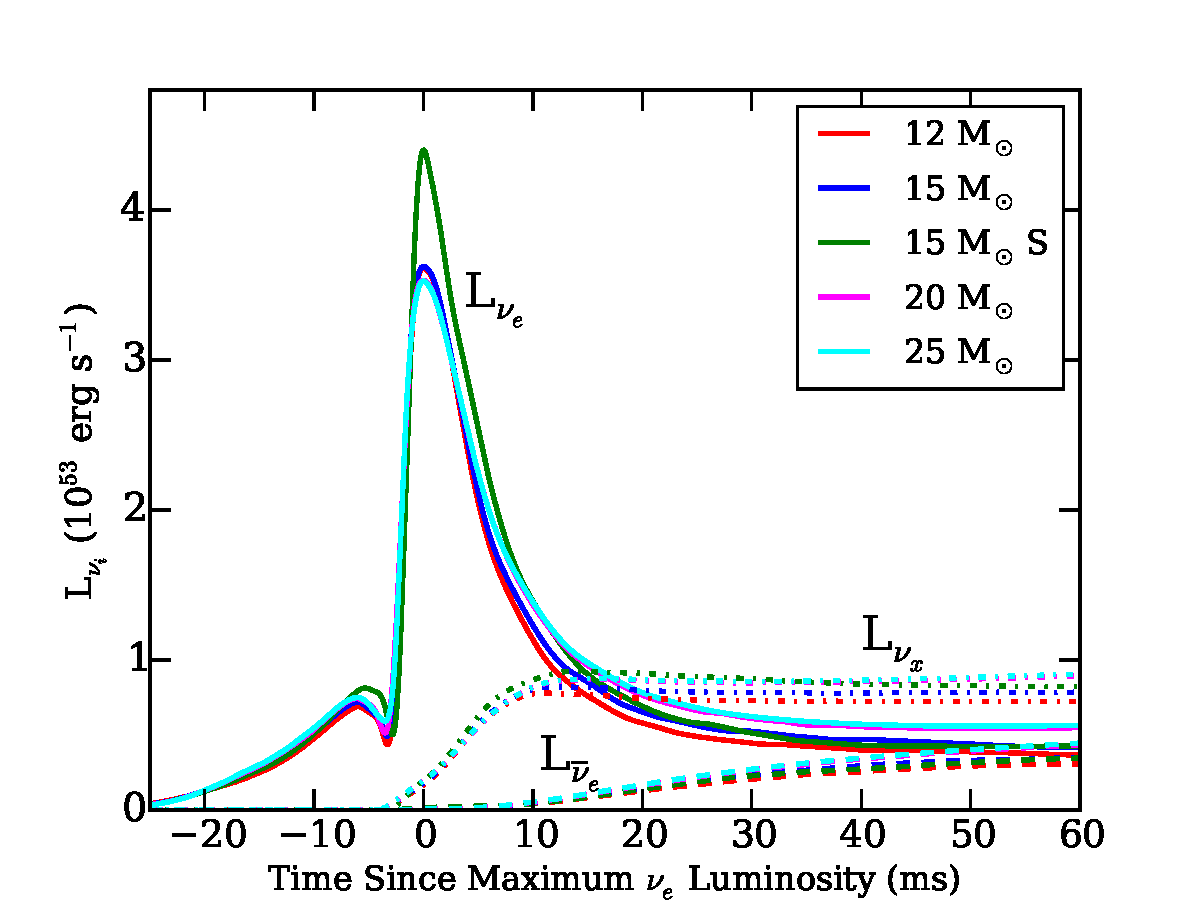
\includegraphics[width=0.7\linewidth]{lum_func_time_outer_radius.pdf}
\caption{\label{fig:lumallt}The unoscillated 
energy luminosity as a function of time for all
three main neutrino channels (\nue, \anue, and \nux) for our five
progenitor 
models.  The solid line represents the \nue\ energy luminosity, the
dashed line represents the \anue\ luminosity, and the dash-dotted line
represents the \nux\ luminosity.  ``S'' designates the \shen\ while
the rest of the models use the \ls\ with $K=220$ MeV. 
Shown is a cubic spline fit to the numerical
data. Time is calculated since the peak of
the \nue\ luminosity.  The \nux\ luminosity is shown for the four
neutrino types ($\nu_\mu,\nu_\tau,\bar\nu_\mu$, and
$\bar\nu_\tau$). The luminosity for any one of these four
neutrino types
will be a quarter the value shown here for \nux.}
\end{figure}

\begin{figure*}[h]
\centering
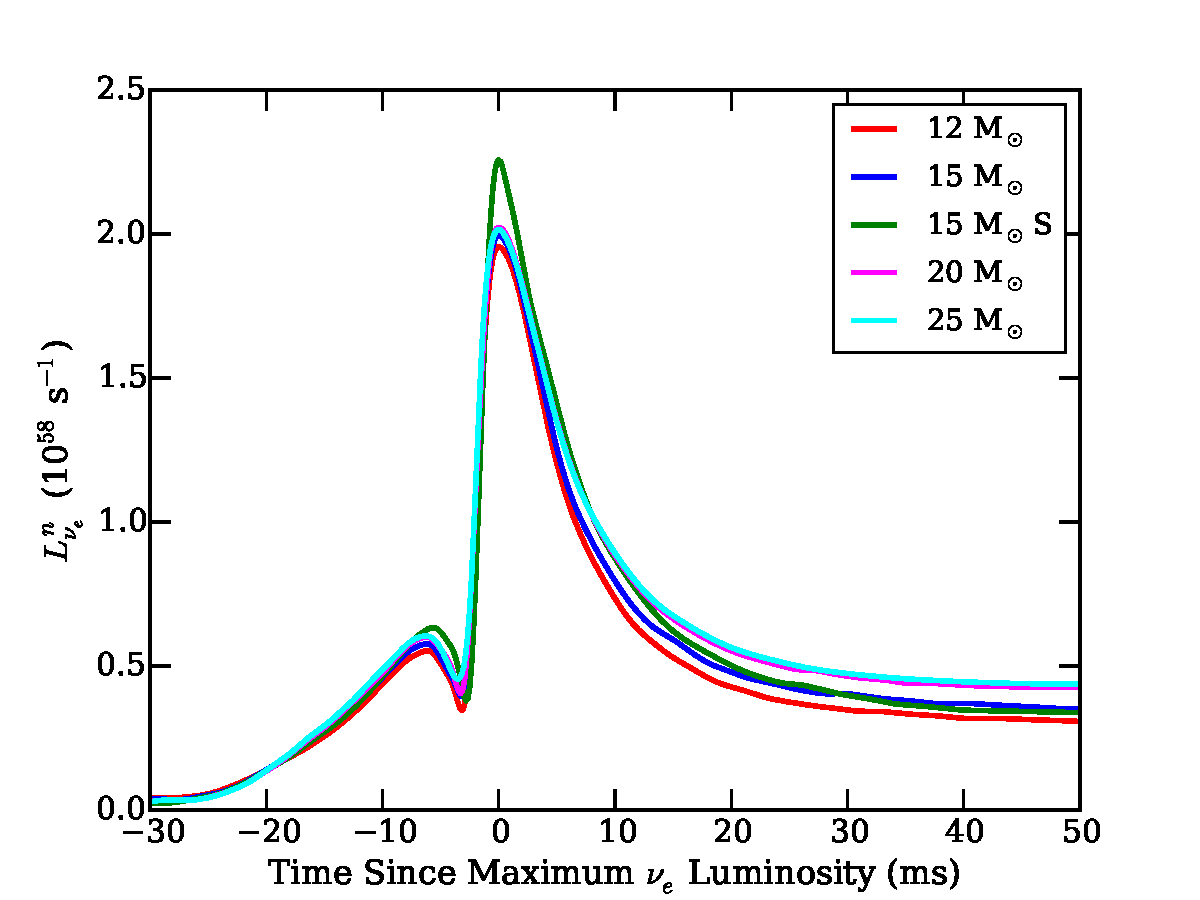
\includegraphics[width=0.75\linewidth]{nue_lum_func_time_all.pdf}
\caption{\label{fig:nuelumt} 
Unoscillated \nue\ number luminosity as a
function of time over breakout for the various models. 
The ``S'' in the figure legend
refers to the \shen; the rest of the models use the \ls\ with $K=220$ MeV.  
The time is centered on the
time of maximum \nue\ luminosity.   The luminosity shows 
two peaks: a small peak on the
initial rise, and a large peak following a sharp rise.  The first,
smaller peak is due to neutrinos from the neutronization of
the collapsing core; the second, larger peak is from \nue's created by
electron capture on free protons liberated by the 
shock. }
\end{figure*}

\begin{figure*}[h]
\centering
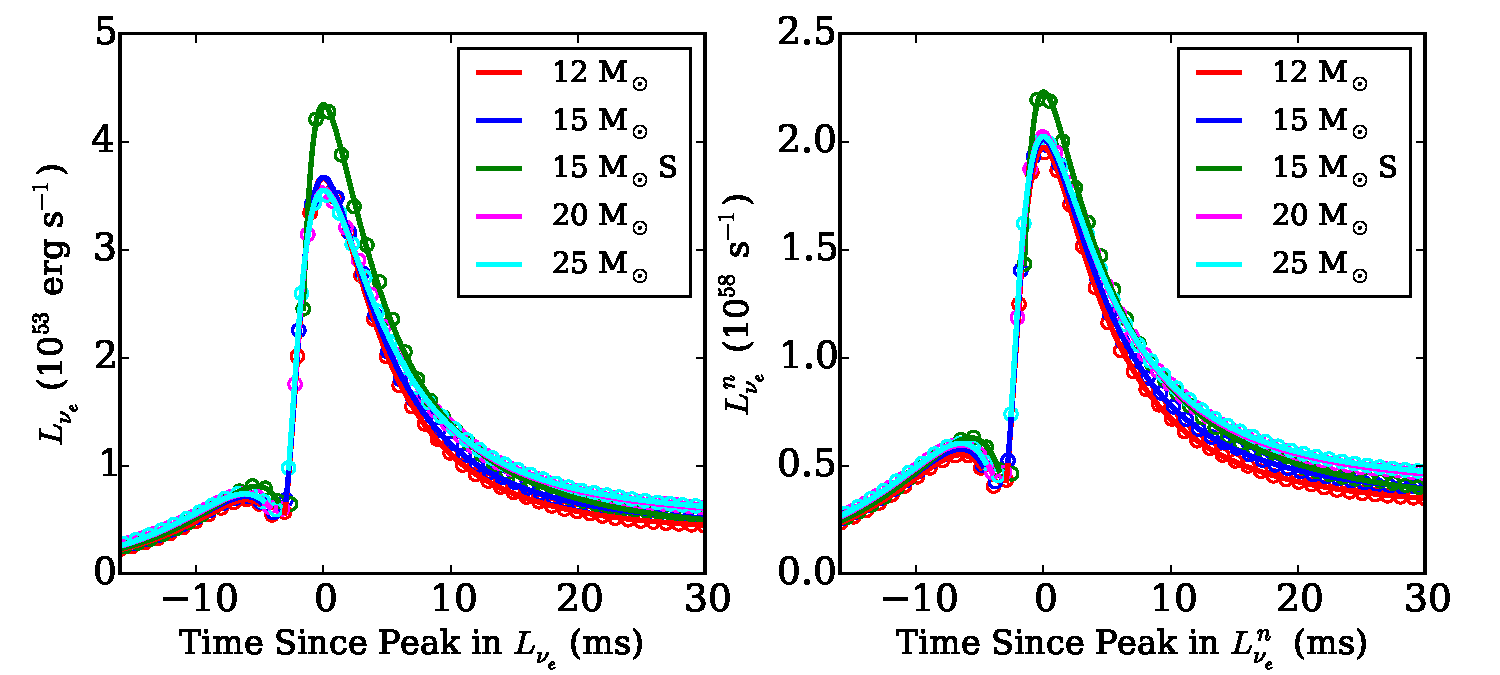
\includegraphics[width=0.85\linewidth]{fittingdemo.pdf}
\caption{\label{fig:fit}Fits to the models, using
  Equations~(\ref{eq:analytic}) and~(\ref{eq:smallpeak}).  
{\it Left}: Fits to the unoscillated energy
  luminosity.  The parameters used in the fits are in
  Tables~\ref{tab:peakfit} and~\ref{tab:smallbumpfit}.
 {\it Right}: Fits to the unoscillated number
  luminosity.  The parameters used in these fits are in
  Tables~\ref{tab:numpeakfit} and~\ref{tab:numsmallbumpfit}.
The numerical model data
  points are shown as circles, while the fits of
  Equations~(\ref{eq:analytic}) and~(\ref{eq:smallpeak})  are shown as
  lines.  For each model, the local minimum between the
  pre-shock neutronization peak and the breakout burst peak is not
  well fit by either of Equations~(\ref{eq:analytic}) and
  ~(\ref{eq:smallpeak}), and so no attempt is made to fit it in this figure.
}
\end{figure*}

\begin{figure*}[h]
\centering
\centerline{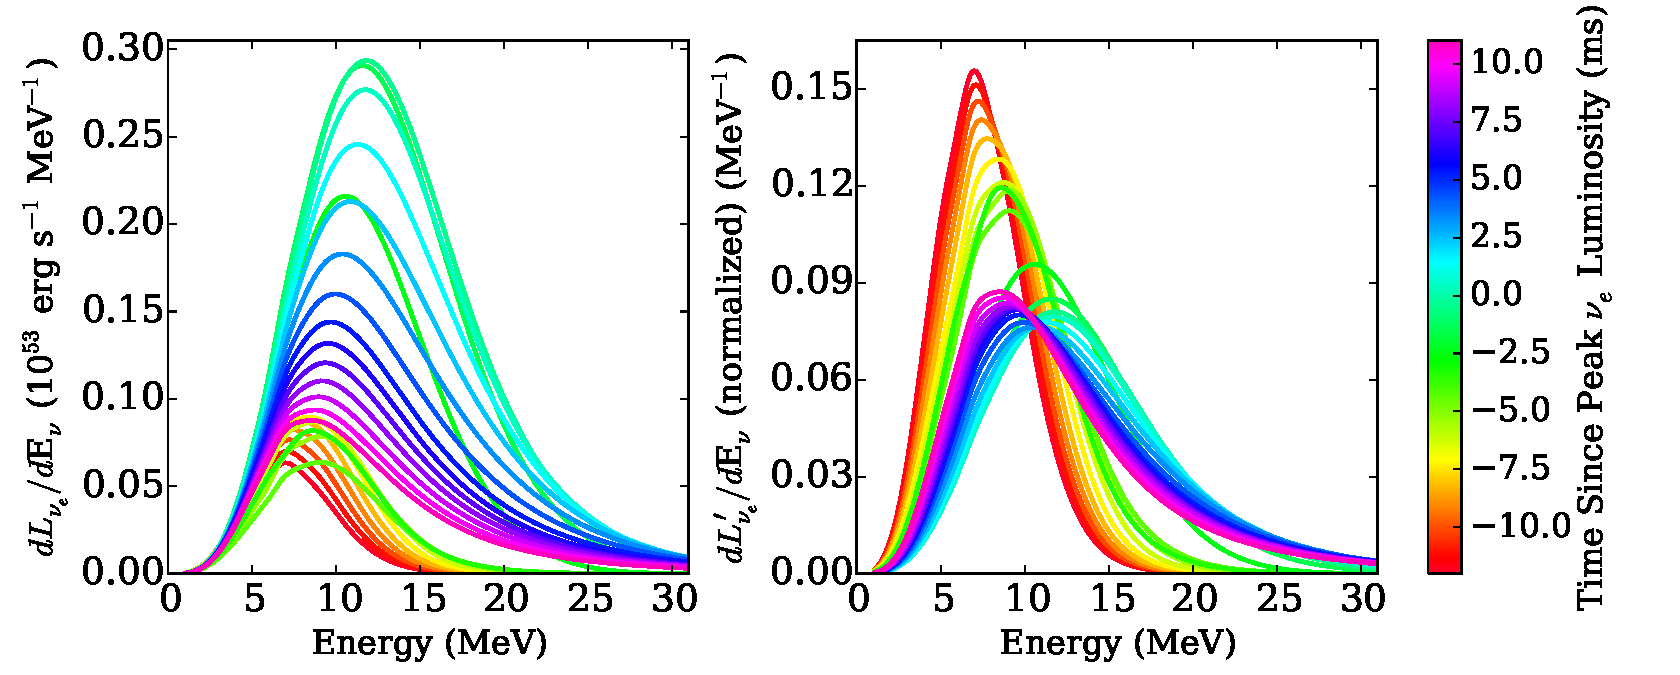
\includegraphics[width=0.95\linewidth]{nue_energy_spectrum_time.pdf}}
\caption{\label{fig:energyspectrum}Unoscillated energy spectra for the 15-\Msol\
  \ls\ model for a range of  times through the breakout burst.  
  Left: the
  full, true spectra.  Right: the normalized spectra, normalized so
  that area under the normalized spectrum of each time (integrated
  over energy) is 1.  Both panels show spectra over the same time range.}
\end{figure*}
%\afterpage{\clearpage}
\begin{figure}[h]
\centering
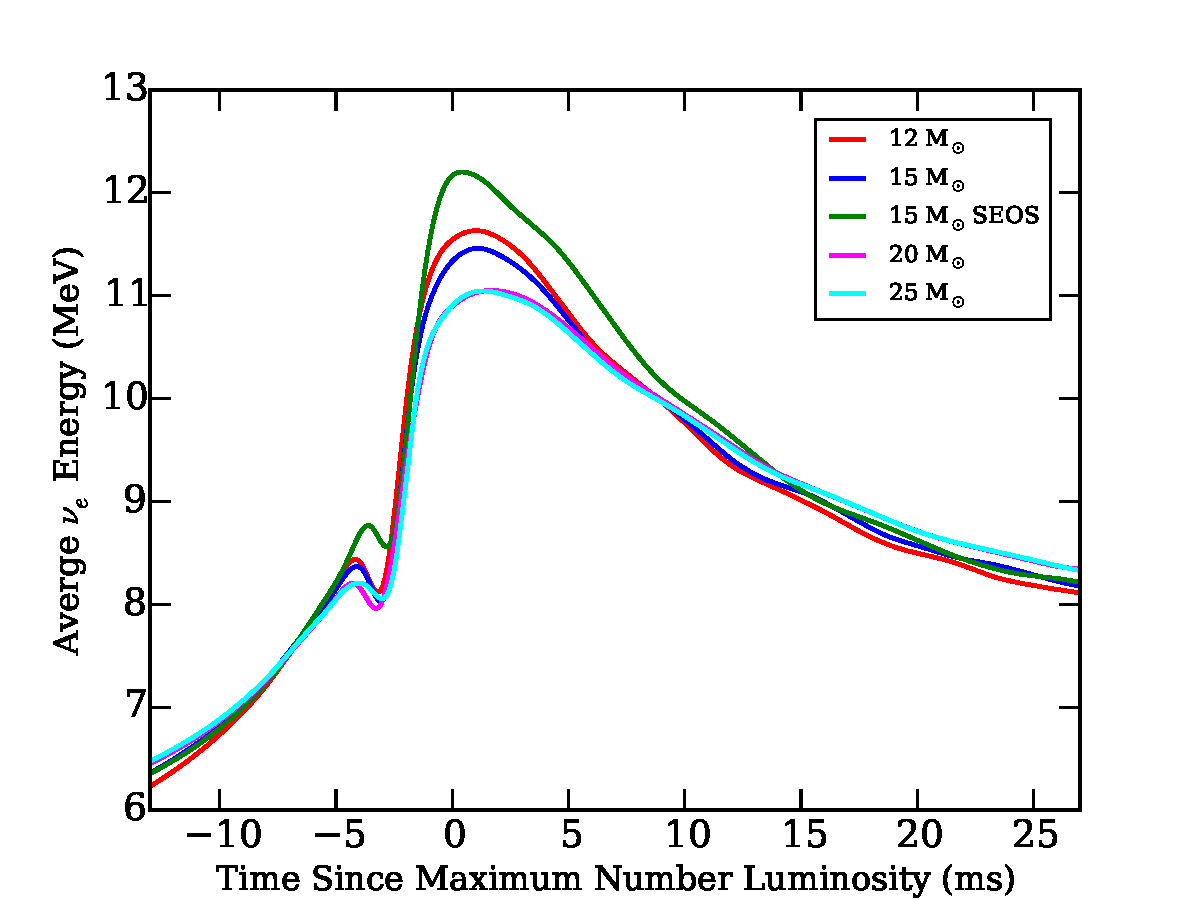
\includegraphics[width=0.65\linewidth]{nue_avg_energy.pdf}
\caption{\label{fig:avgenergy}Average \nue\ energy as a function of
time shown for all the models through the breakout burst. The average
energy is defined by Equation~(\ref{eq:averageenergy}).  Time is
calculated as time since maximum number luminosity for the fits to the
number luminosity for each model.  For the same 
equation of state, the peak average energy decreases with progenitor
mass down to 20 \Msol, with the 20- and 25-\Msol\ progenitors
showing comparable values, while the average energy in the tail after 
peak increases with progenitor mass (again, with the 20-  and 
25-\Msol\ progenitors
showing comparable values).
The models show a smaller peak in average energy, which is 
associated with the 
pre-breakout neutronization peak. 
The 15-\Msol\ \shen\ model has a slightly higher average
average energy during both the breakout burst peak and pre-shock
neutronization peak compared to its \ls\
counterpart, but comparable average energy coming into and leaving the
breakout burst.  The average energy for all the models peaks at a time
slightly after the
time of maximum number luminosity.} 
\end{figure}

%Figure 6
\begin{figure}[h]
\centering
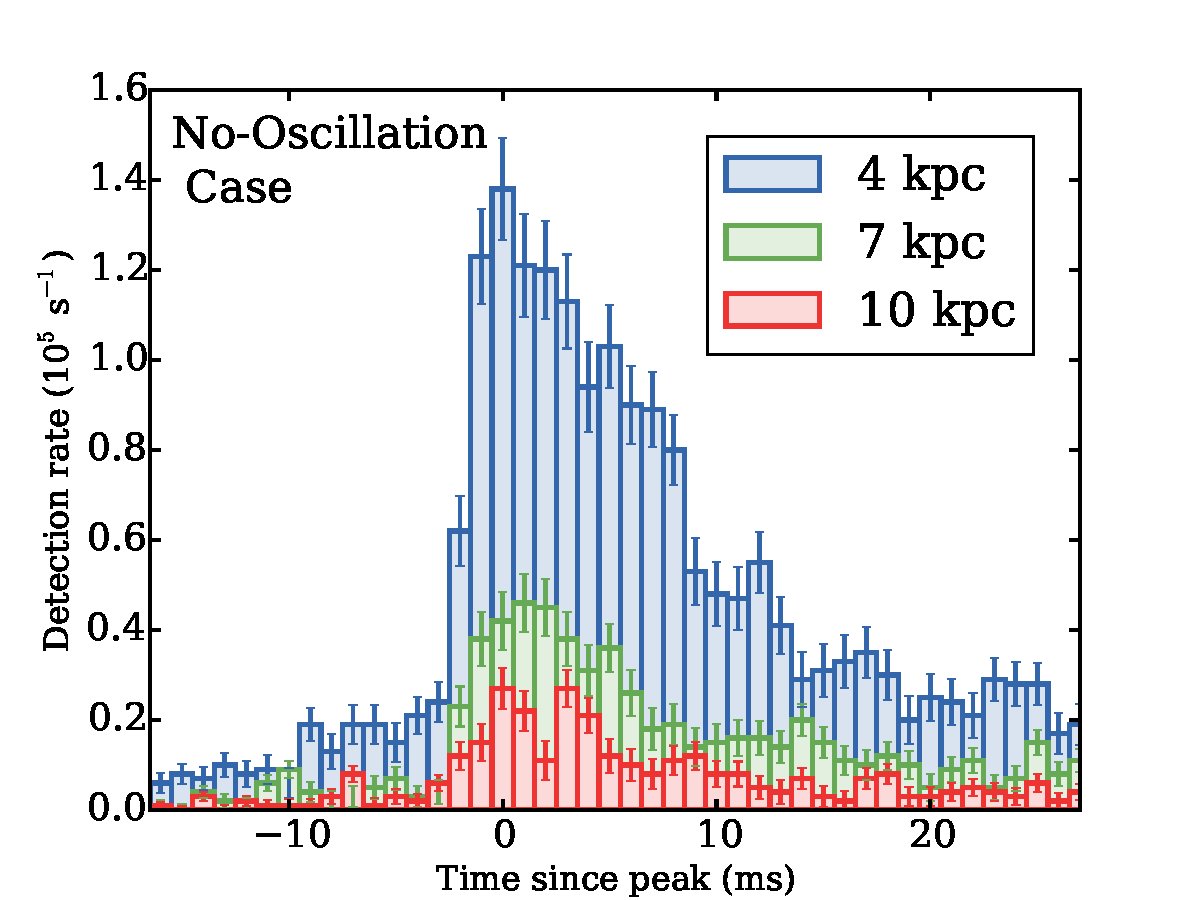
\includegraphics[width=0.7\linewidth]{hyperk_histograms.pdf}
\caption{\label{fig:hyperkhistogram}Example realization of detection
  rates in the no-oscillation case with
  1$\sigma$ error bars for CCSN neutrino detections in
  Hyper-K at distances of 4, 7, and 10 kpc, binned in 1-ms time bins.
  This figure shows not only the overall increase in signal expected
  in Hyper-K as the distance to the supernova decreases, but also gives a
  general sense of how the expected noise and error bars in each time bin
  depend on $D$.}
\end{figure}
%\afterpage{\clearpage}

%\begin{figure*}[h]
%\centerline{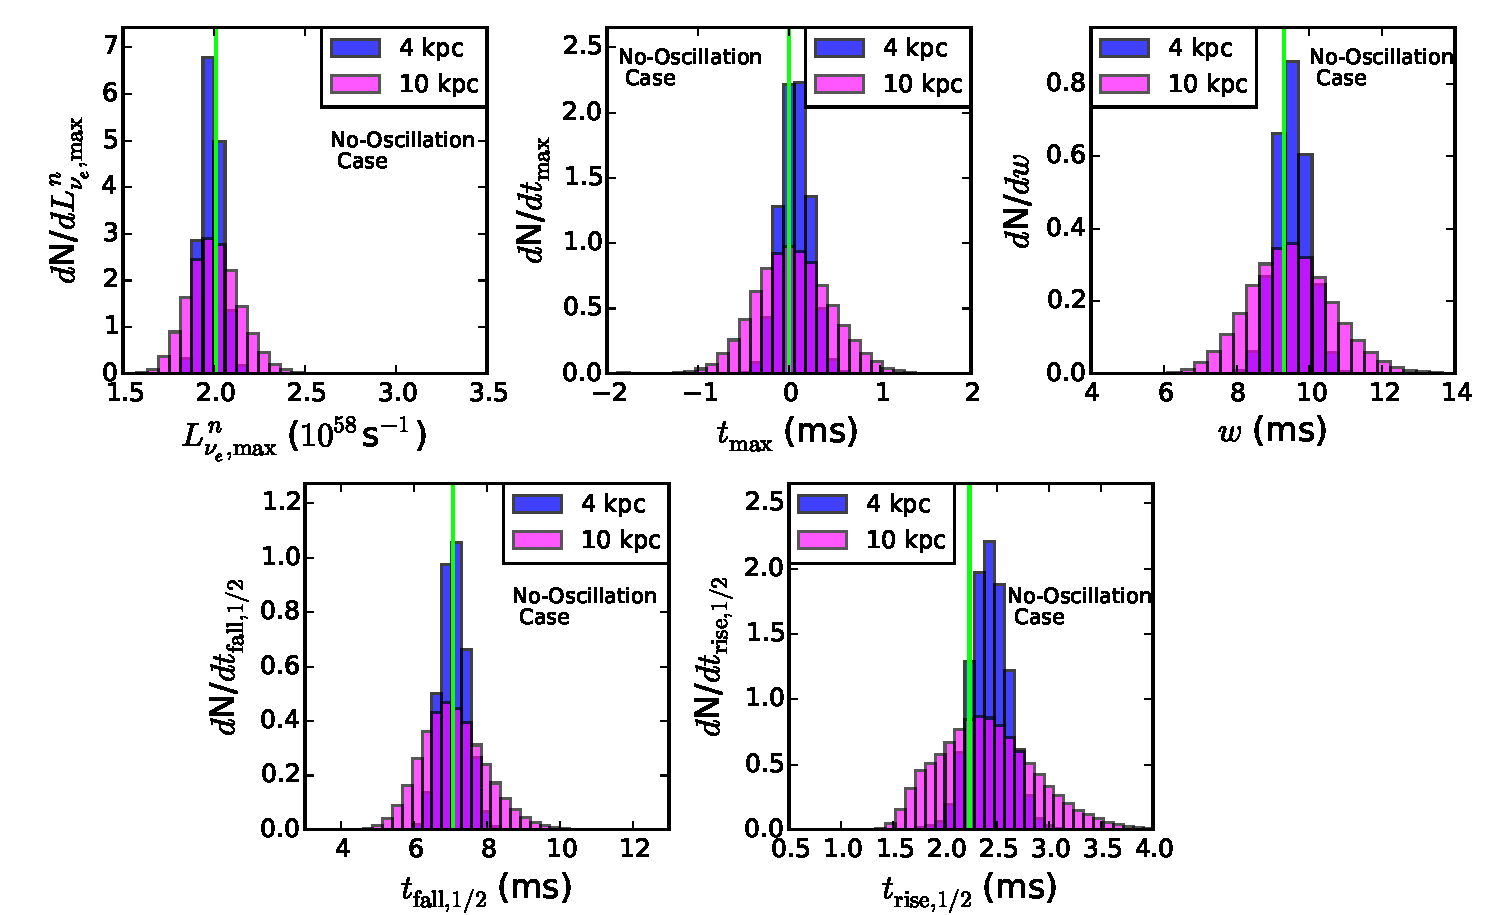
\includegraphics[width=.943\linewidth]{wh07_15_40g_IceCube_realparameters_histogram.pdf}}
%\caption{\label{fig:icecubephysicalparms_hist} Probability density
% functions  for the physical
%  parameters derived from fits of Equation~(\ref{eq:analytic}) to the 
%simulated observations for IceCube for the 
%15-\Msol\ \ls\ model in the no-oscillation case.  
%For each parameter, blue shows the 
%probability density function corresponding to a supernova
%at a distance of 4 kpc and magenta shows the probability density function
%corresponding to a supernova at a distance of
%10 kpc.  Overlap between the two probability density 
%functions is shown as purple.  The
%model value is shown as a green vertical line.}
%\end{figure*}

%\afterpage{\clearpage}
\begin{figure*}[h]
\centerline{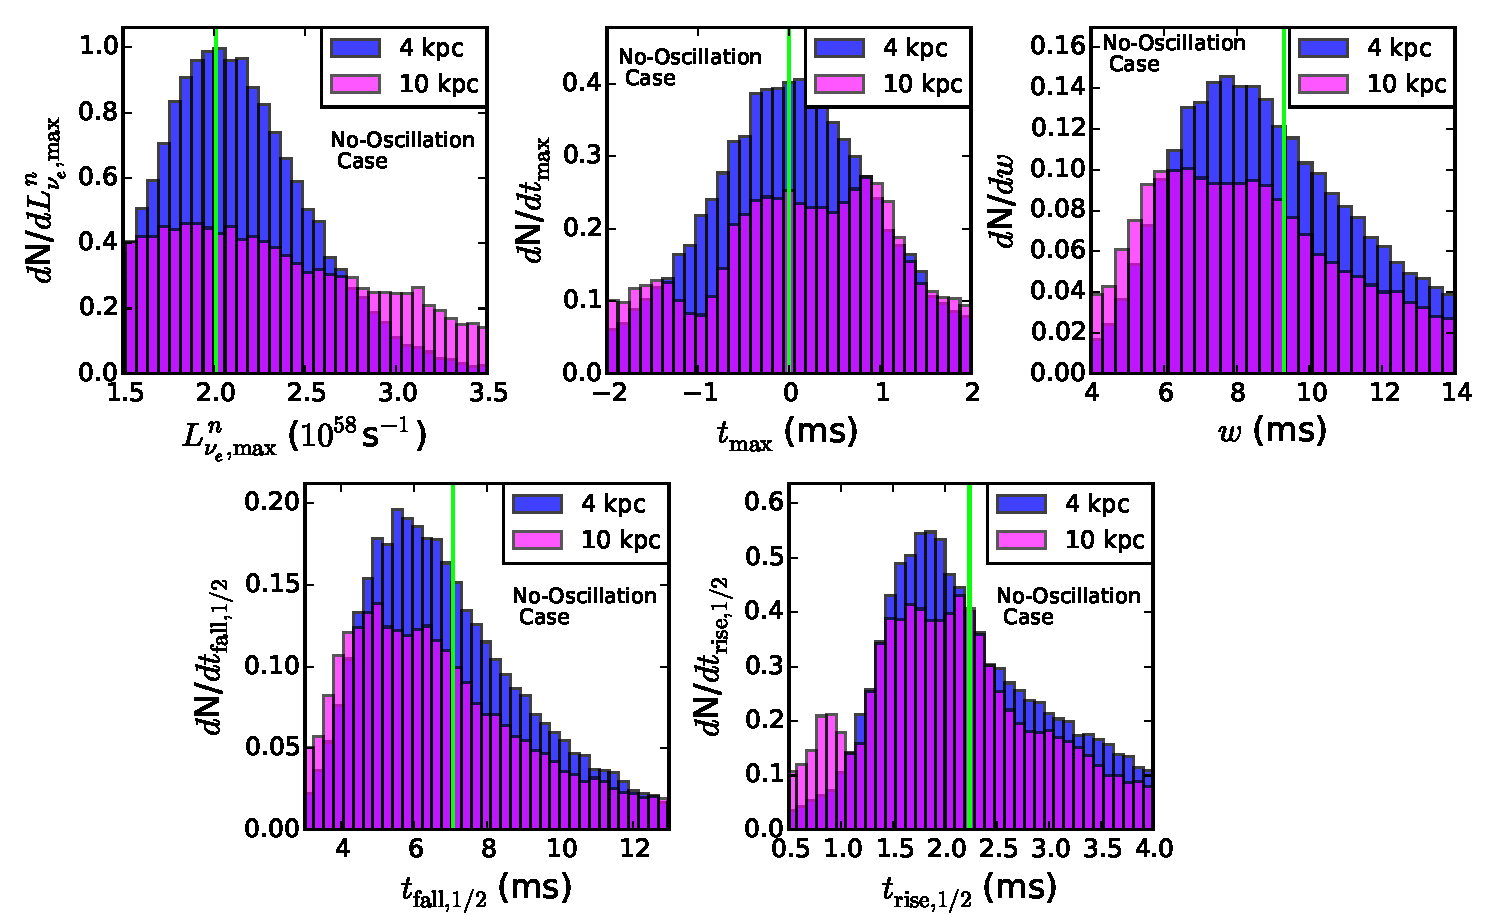
\includegraphics[width=.943\linewidth]{wh07_15_40g_SuperK_realparameters_histogram.pdf}}
\caption{\label{fig:superkphysicalparms_hist} 
 Probability density
 functions  for the physical
  parameters derived from fits of Equation~(\ref{eq:analytic}) to the 
simulated observations for Super-K for the 
15-\Msol\ \ls\ model in the no-oscillation case.  
For each parameter, blue shows the 
probability density function corresponding to a supernova
at a distance of 4 kpc and magenta shows the probability density function
corresponding to a supernova at a distance of
10 kpc.  Overlap between the two probability density 
functions is shown as purple.  The
model value is shown as a green vertical line.}
\end{figure*}


\begin{figure*}[h]
\centerline{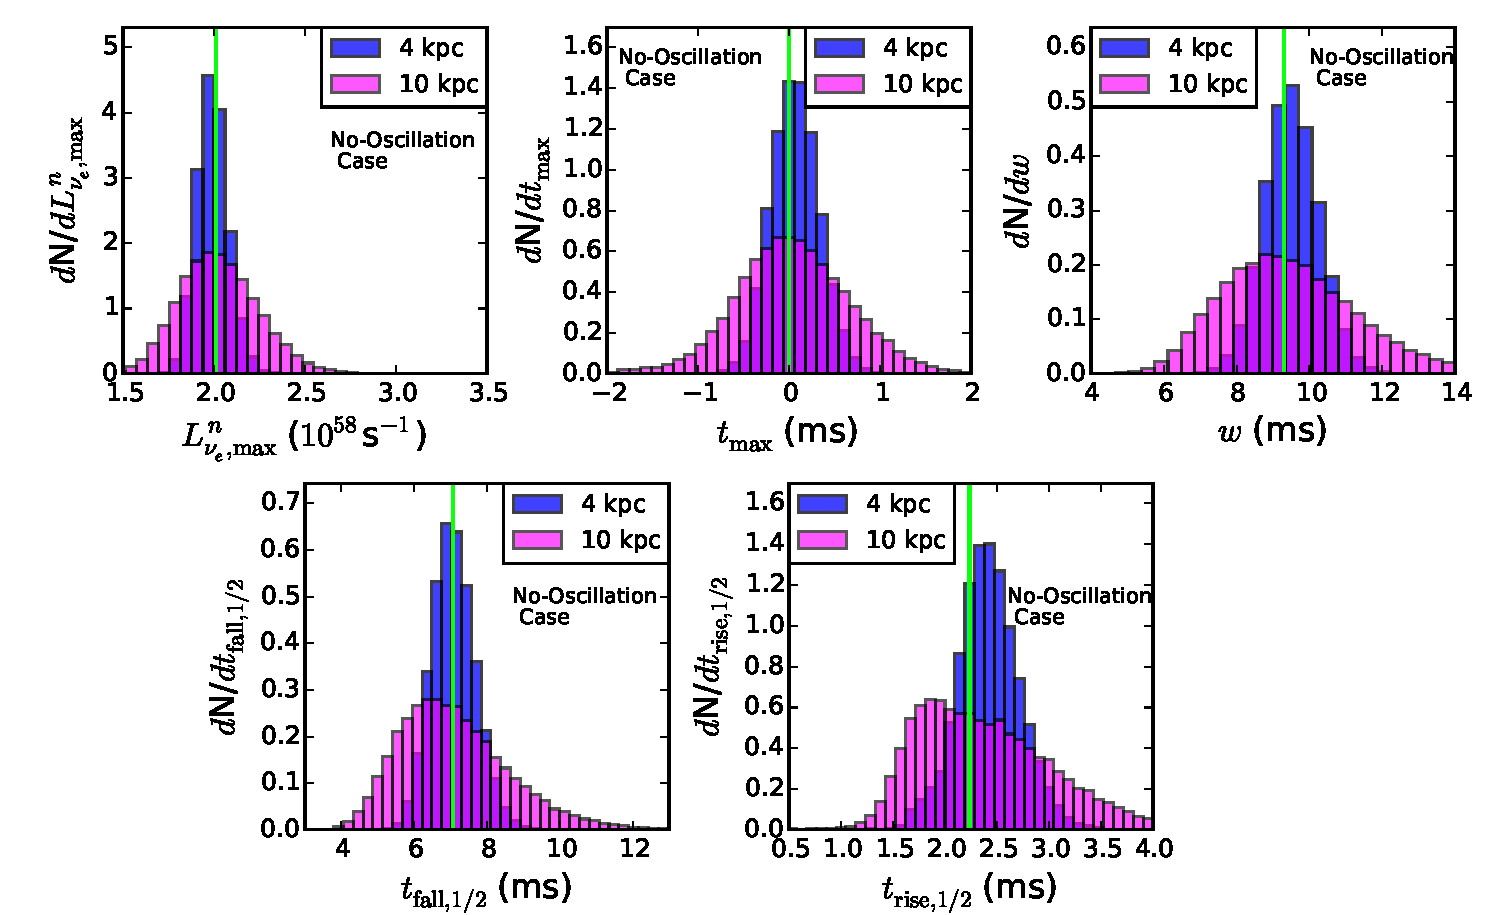
\includegraphics[width=0.943\linewidth]{wh07_15_40g_HyperK_realparameters_histogram.pdf}}
\caption{\label{fig:hyperkphysicalparms_hist} Same as
  Figure~\ref{fig:superkphysicalparms_hist}, but for Hyper-K in the
  no-oscillation case.}
\end{figure*}


%\afterpage{\clearpage}

%Figure 10
\begin{figure*}[h]
\centerline{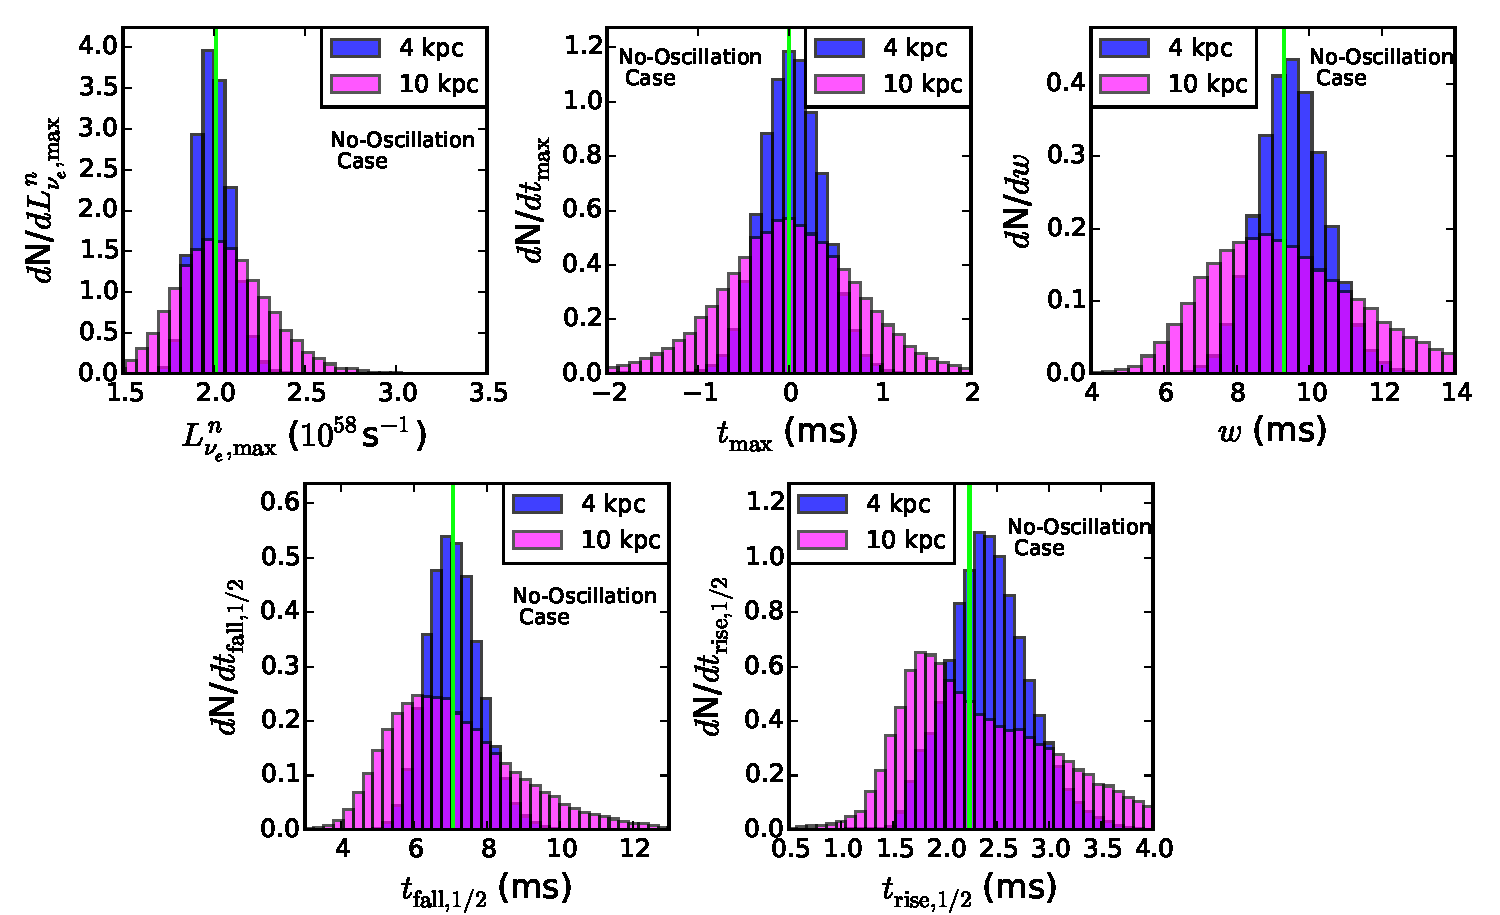
\includegraphics[width=0.943\linewidth]{wh07_15_40g_DUNE_realparameters_histogram.pdf}}
\caption{\label{fig:dunephysicalparms_hist} Same as
  Figure~\ref{fig:superkphysicalparms_hist}, but for DUNE in the
  no-oscillation case.}
\end{figure*}


\begin{figure*}[h]
\centerline{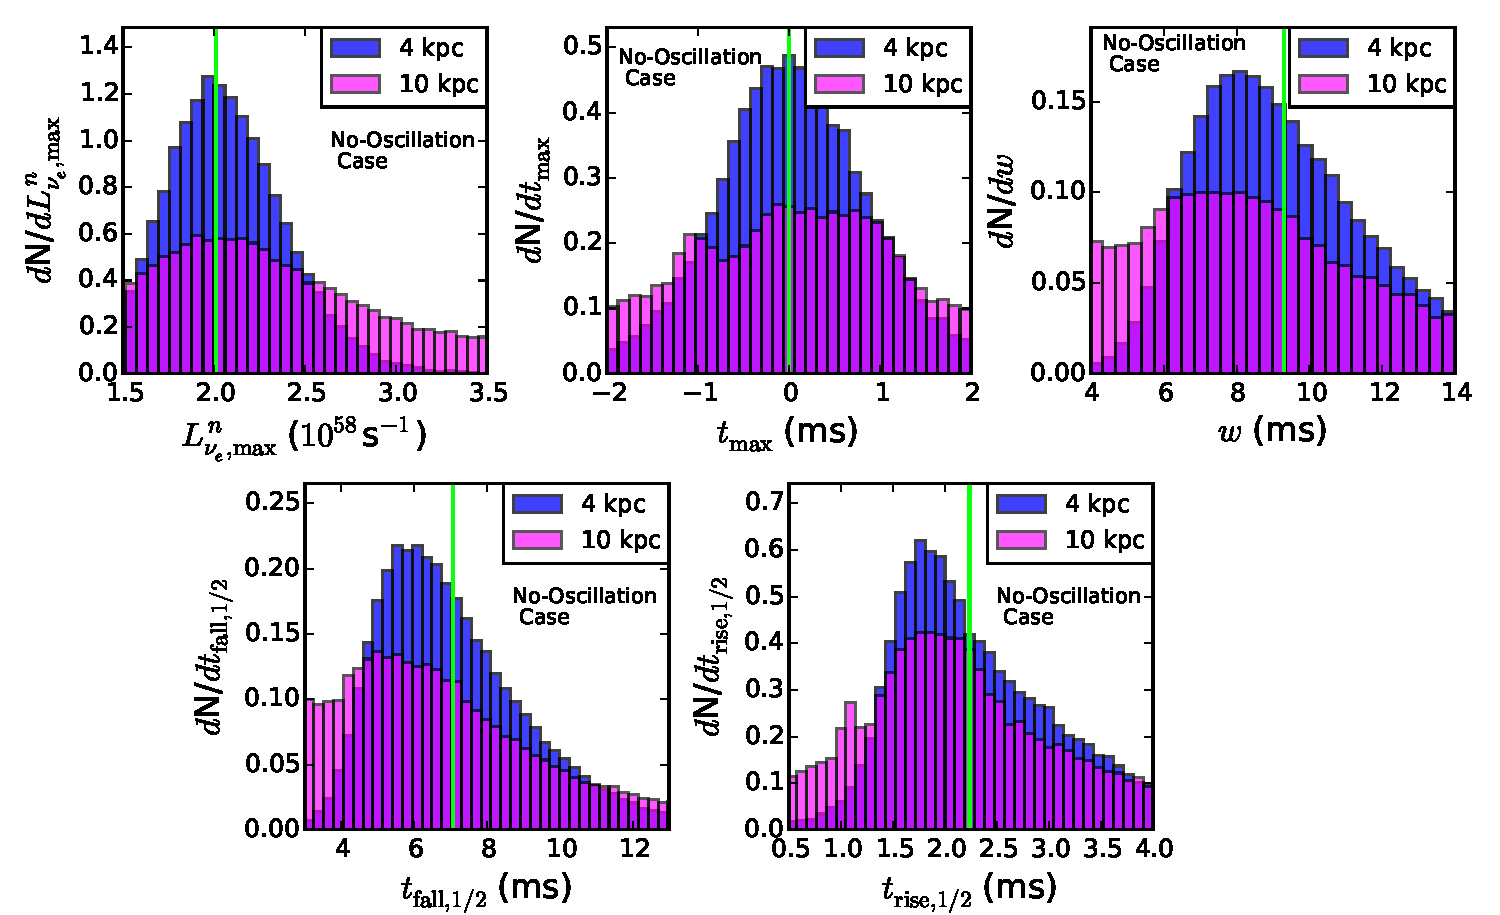
\includegraphics[width=0.943\linewidth]{wh07_15_40g_JUNO_realparameters_histogram.pdf}}
\caption{\label{fig:junophysicalparms_hist} Same as
  Figure~\ref{fig:superkphysicalparms_hist}, but for JUNO in the
  no-oscillation case.}
\end{figure*}

%\afterpage{\clearpage}

\begin{figure*}[h]
\centerline{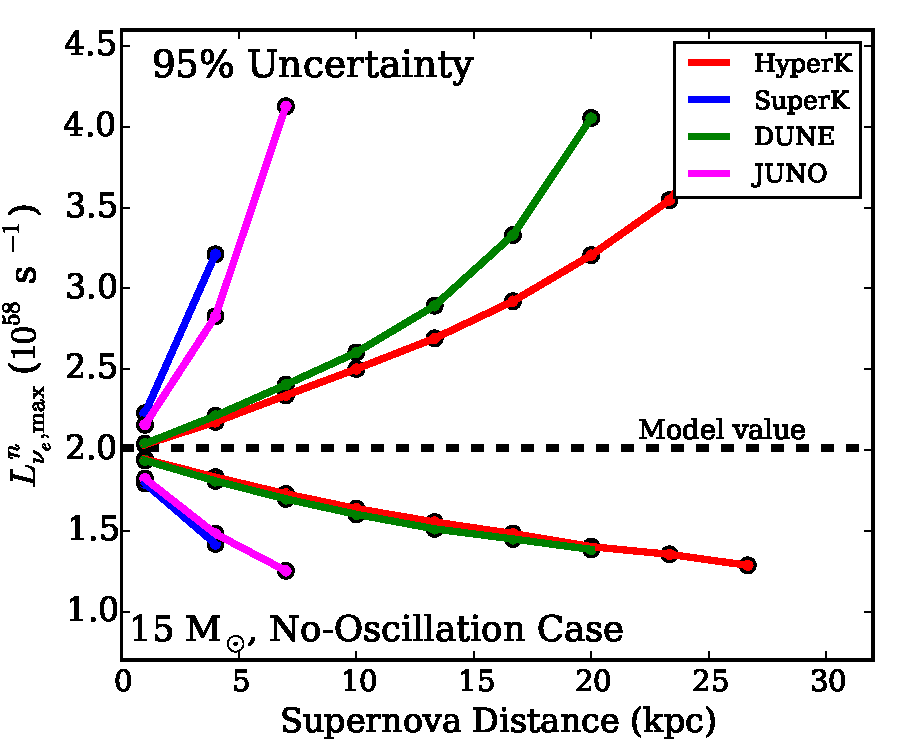
\includegraphics[width=.6\linewidth]{wh07_15_40g_parametergroup_0_95_funcdistance.pdf}}
\caption{\label{fig:15maxvalfuncD} The 95\% uncertainty in measuring \lmax\ as a
  function of distance for various detectors for the 15
  \Msol\ \ls\ model, in the no-oscillation case. For each detector, the lines represent the span
  needed to include 95\% of the \lmax's calculated from the set of
  $5\times10^4$ 
  sampled observations. 
 When the uncertainty values for a
  specific detector get either
  too large or too small relative to the model value, we stop plotting
  the uncertainty at that distance and greater distances.  The uncertainty values for 
Super-K and JUNO were cut off
  at 7 kpc if the previous criteria were not met at 7 kpc because of
  the small number of events for a supernova beyond that
  distance.
}
\end{figure*}

%\afterpage{\clearpage}

\begin{figure*}[h]
\centerline{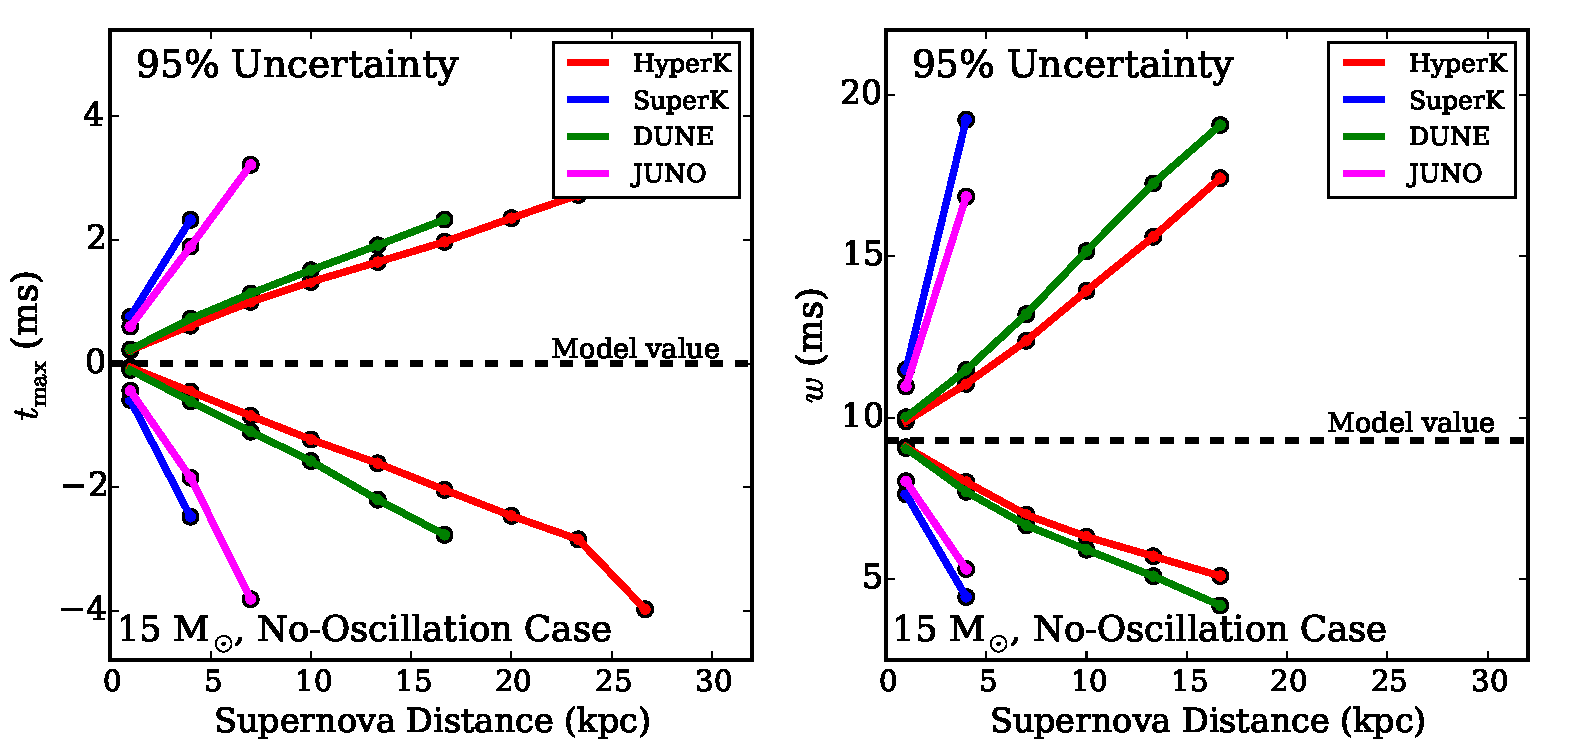
\includegraphics[width=\linewidth]{wh07_15_40g_parametergroup_1_95_funcdistance.pdf}}
\caption{\label{fig:15maxlocfwhmfuncD} Same as
  Figure~\ref{fig:15maxvalfuncD}, but for {\it Left}: \tmax, and {\it
    Right}: $w$, in the no-oscillation case.}
\end{figure*}

\begin{figure*}[h]
\centerline{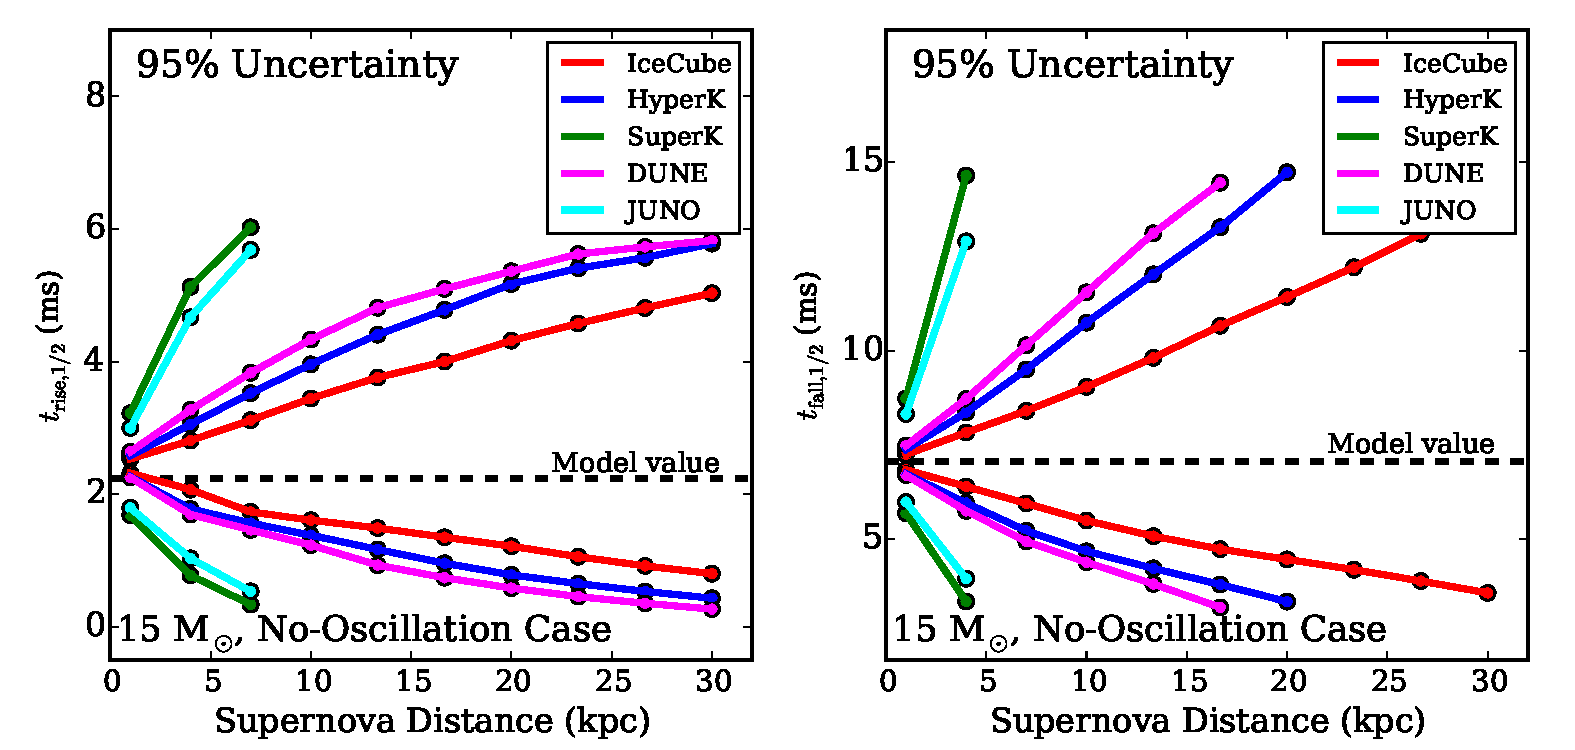
\includegraphics[width=\linewidth]{wh07_15_40g_parametergroup_2_95_funcdistance.pdf}}
\caption{\label{fig:15lwhmrwhmfuncD} Same as
  Figure~\ref{fig:15maxvalfuncD}, but for {\it Left}: \trise, and {\it
    Right}: \tfall, in the no-oscillation case.}
\end{figure*}


\afterpage{\clearpage}

%Figure 15
\begin{figure*}[*h]
\centerline{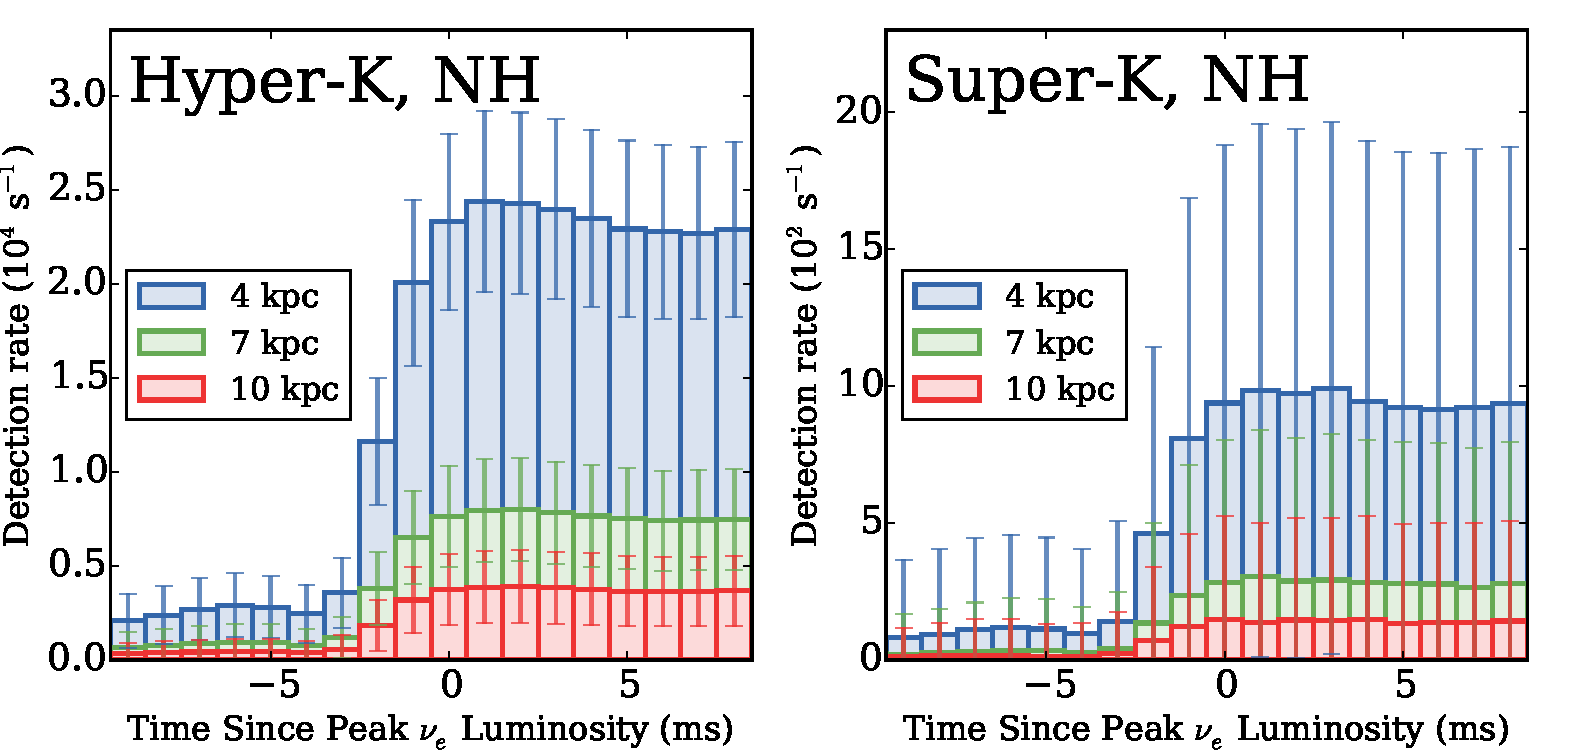
\includegraphics[width=\linewidth]{backgrounds_histogram_groupingnumber_0_NH.pdf}}
\caption{\label{fig:hyperk_superk_juno_nh_backgrounds} {\it Left}: For Hyper-K,
  {\it Middle}: for Super-K, and {\it Right}: for JUNO, the expected light curve
  for supernovae at 4, 7, and 10 kpc, incorporating the neutrino
  oscillations expected in the case of the NH.  Detections of neutrinos of all
  flavors are taken into account, with (for Hyper-K and Super-K) IBD's and NC scattering off of oxygen
  subtracted, and (for JUNO) IBD's and NC scattering off of carbon
  subtracted.  Each time bin shows the mean
  count rate in that time bin over 10$^4$ realizations and the error
  bars show the standard deviation based on the same 10$^4$
  realizations.}
\end{figure*}

%\clearpage

\begin{figure*}[h]
\centerline{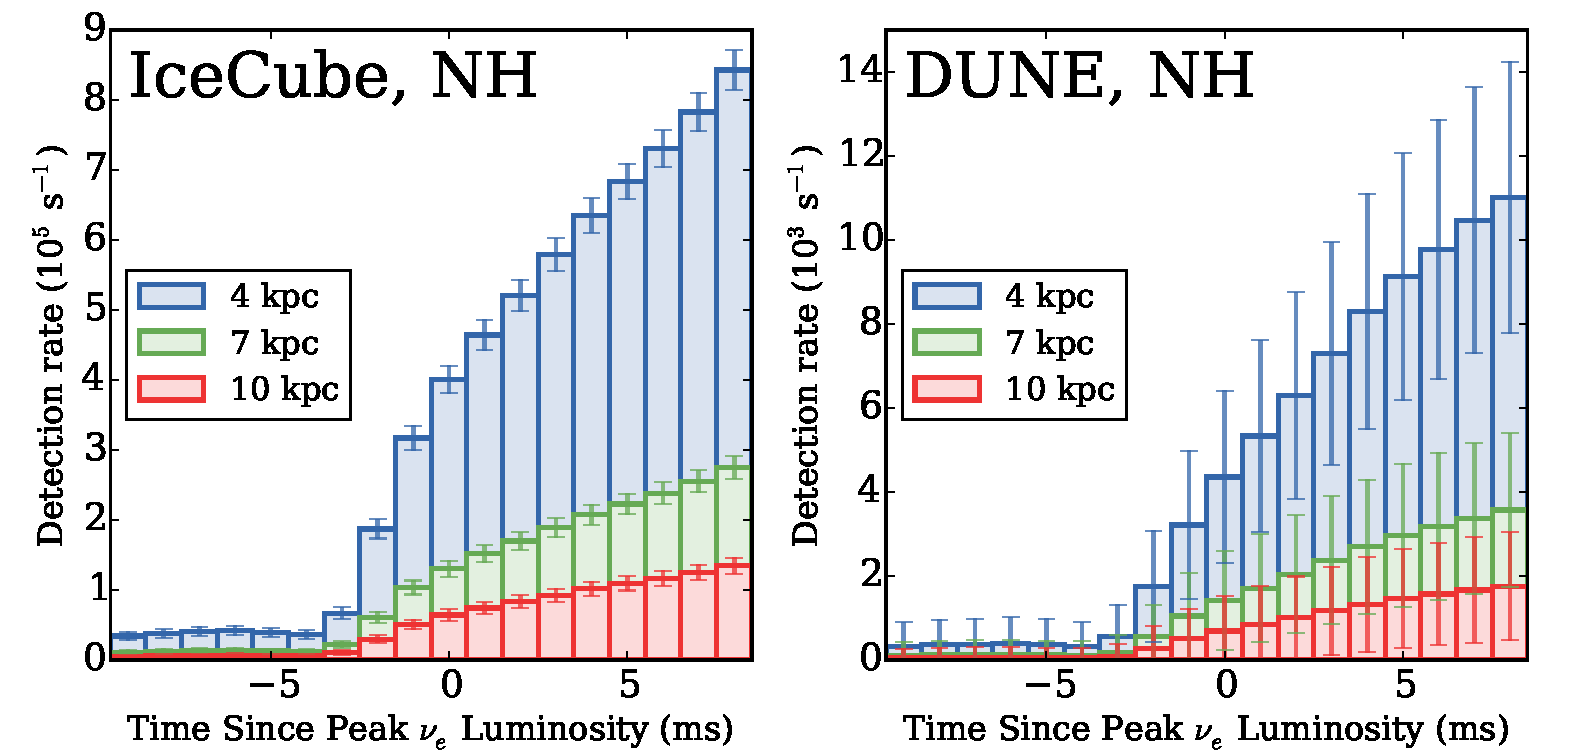
\includegraphics[width=\linewidth]{backgrounds_histogram_groupingnumber_1_NH.pdf}}
\caption{\label{fig:icecube_dune_nh_backgrounds} Similar to
  Figure~\ref{fig:hyperk_superk_juno_nh_backgrounds}, but for {\it Left}:
  IceCube and {\it Right}: DUNE. No signals from any detection channel
  have been subtracted.
}
\end{figure*}

%\clearpage

%%IH
\begin{figure*}[h]
\centerline{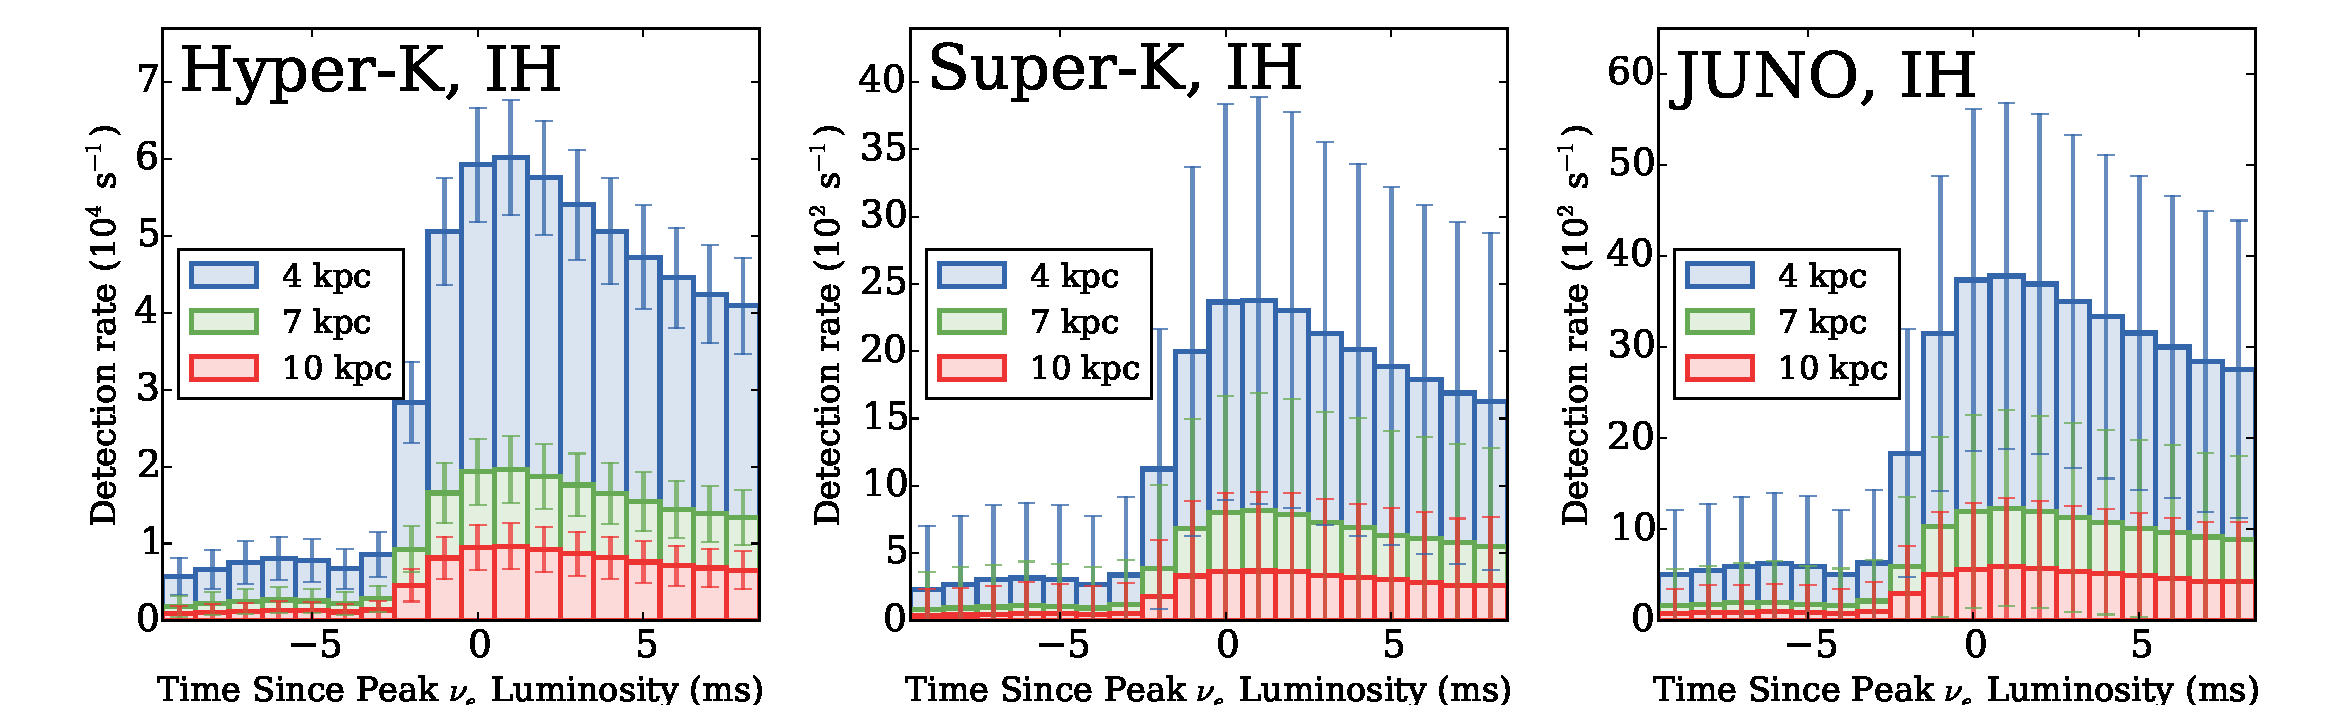
\includegraphics[width=\linewidth]{backgrounds_histogram_groupingnumber_0_IH.pdf}}
\caption{\label{fig:hyperk_superk_juno_ih_backgrounds} Similar to 
  Figure~\ref{fig:hyperk_superk_juno_nh_backgrounds}, but using the neutrino
  oscillations expected for the IH instead of the NH.
}
\end{figure*}


\begin{figure*}[h]
\centerline{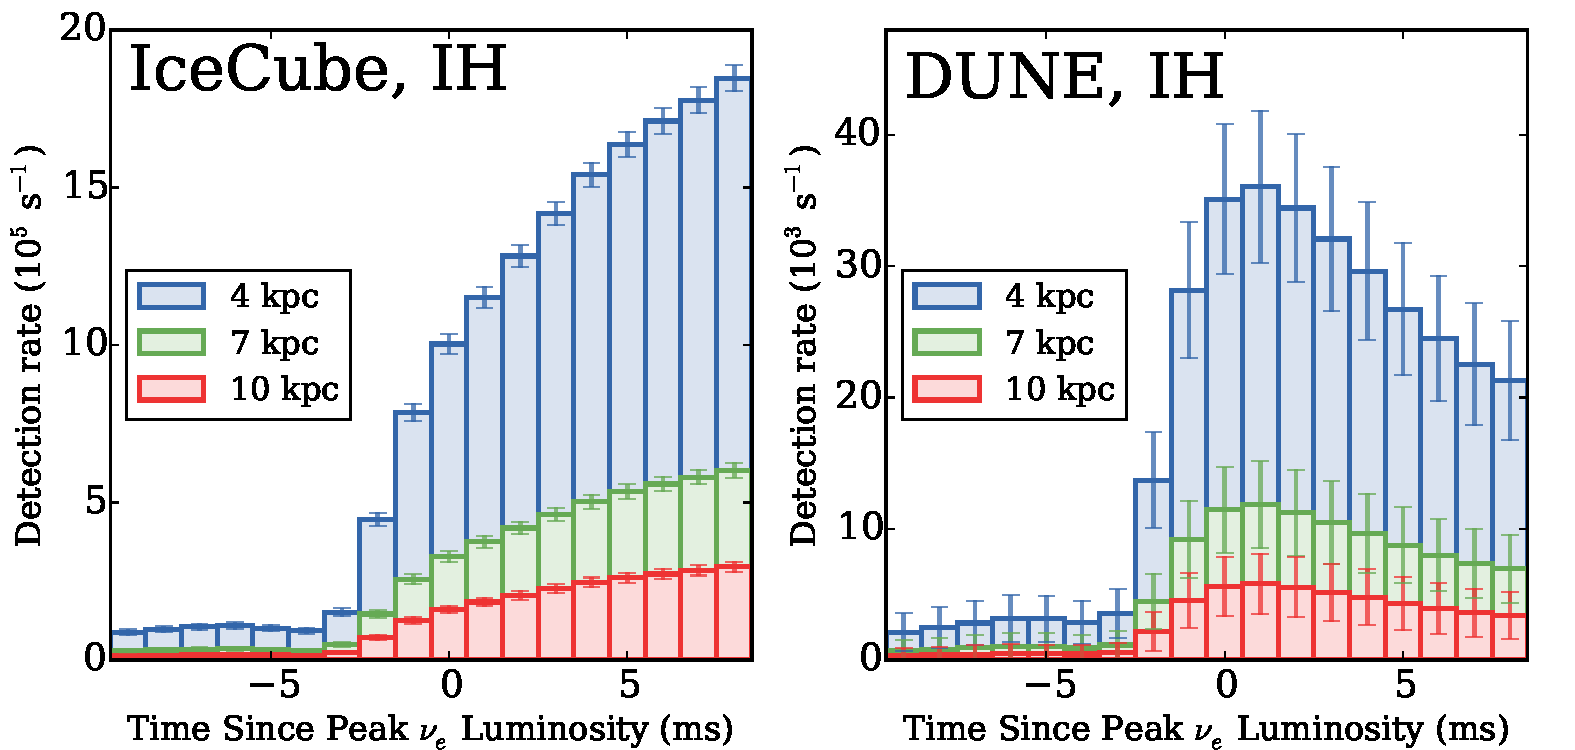
\includegraphics[width=\linewidth]{backgrounds_histogram_groupingnumber_1_IH.pdf}}
\caption{\label{fig:icecube_dune_ih_backgrounds} Similar to
  Figure~\ref{fig:icecube_dune_nh_backgrounds}, but using the neutrino
  oscillations expected for the IH instead of the NH.
}
\end{figure*}


%Figure 19
\begin{figure*}[h]
\centerline{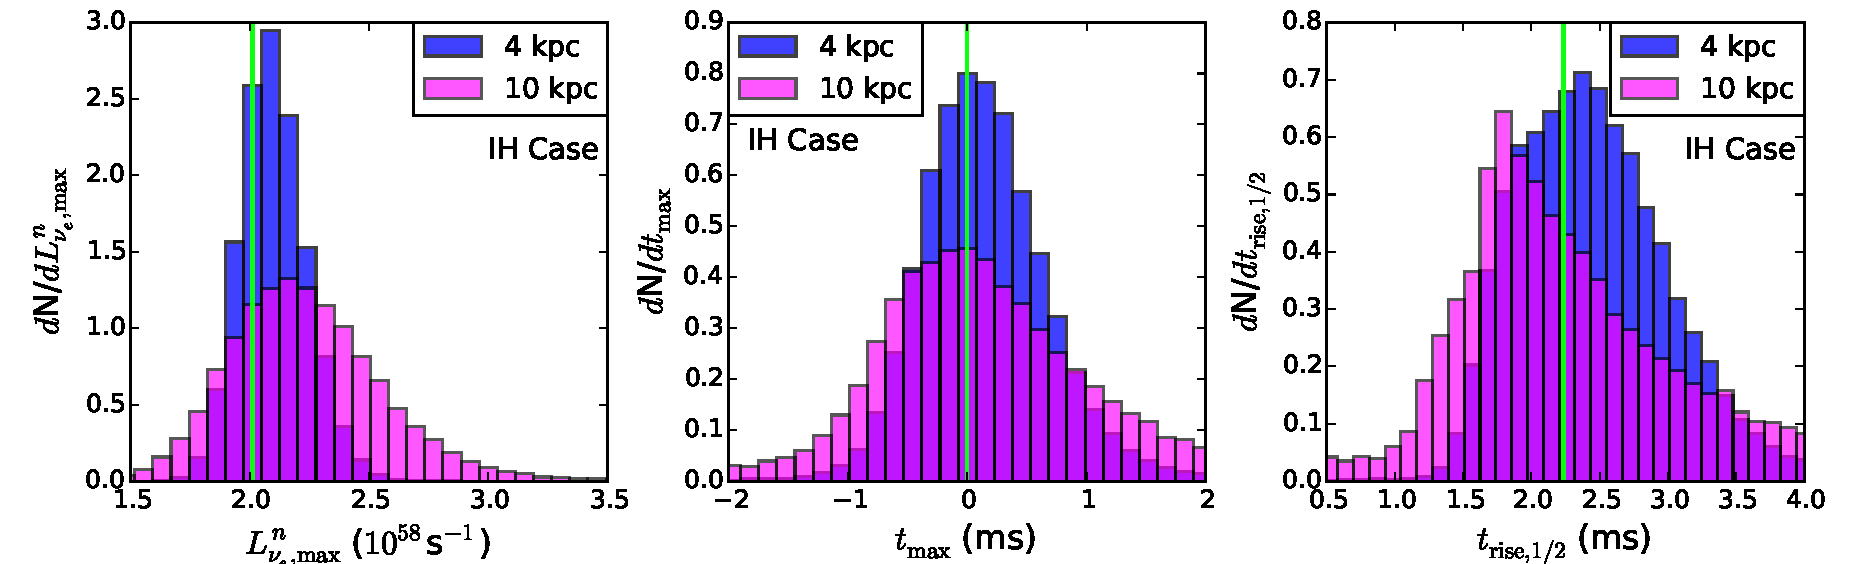
\includegraphics[width=\linewidth]{wh07_15_40g_HyperK_realparameters_histogram_oscillations_backgrounds_IH.pdf}}
\caption{\label{fig:hyperkphysicalparms_hist_ih} Same as
  Figure~\ref{fig:hyperkphysicalparms_hist}, but for the IH case and
  with only \lmax, \tmax, and \trise\ shown.  For Hyper-K, the
  background signals due to IBD's and NC scatterings off of oxygen
  have been subtracted.}
\end{figure*}


\begin{figure*}[h]
\centerline{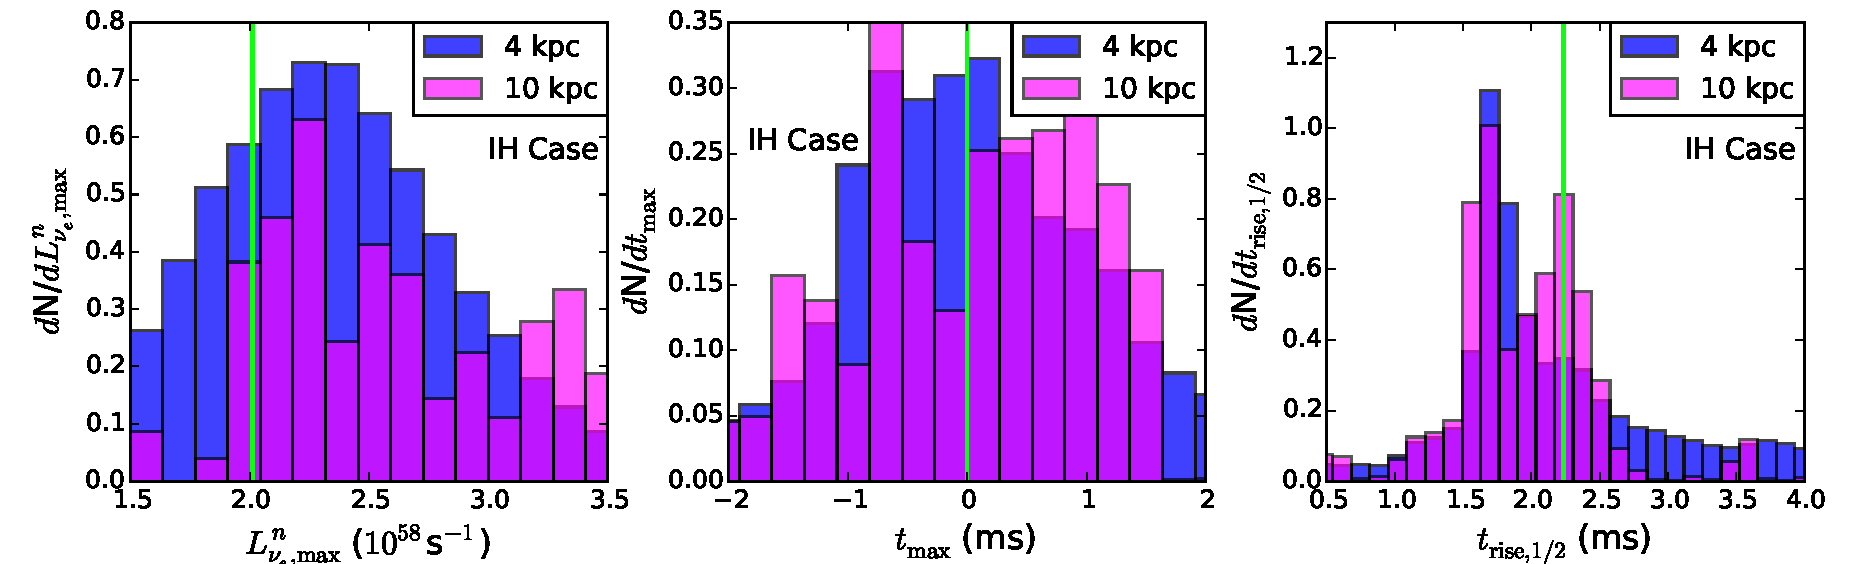
\includegraphics[width=\linewidth]{wh07_15_40g_SuperK_realparameters_histogram_oscillations_backgrounds_IH.pdf}}
\caption{\label{fig:superkphysicalparms_hist_ih} Same as
  Figure~\ref{fig:hyperkphysicalparms_hist_ih}, but for Super-K in the
  IH case.  For Super-K, the
  background signals due to IBD's and NC scatterings off of oxygen
  have been subtracted.}
\end{figure*}
\afterpage{\clearpage}

\begin{figure*}[h]
\centerline{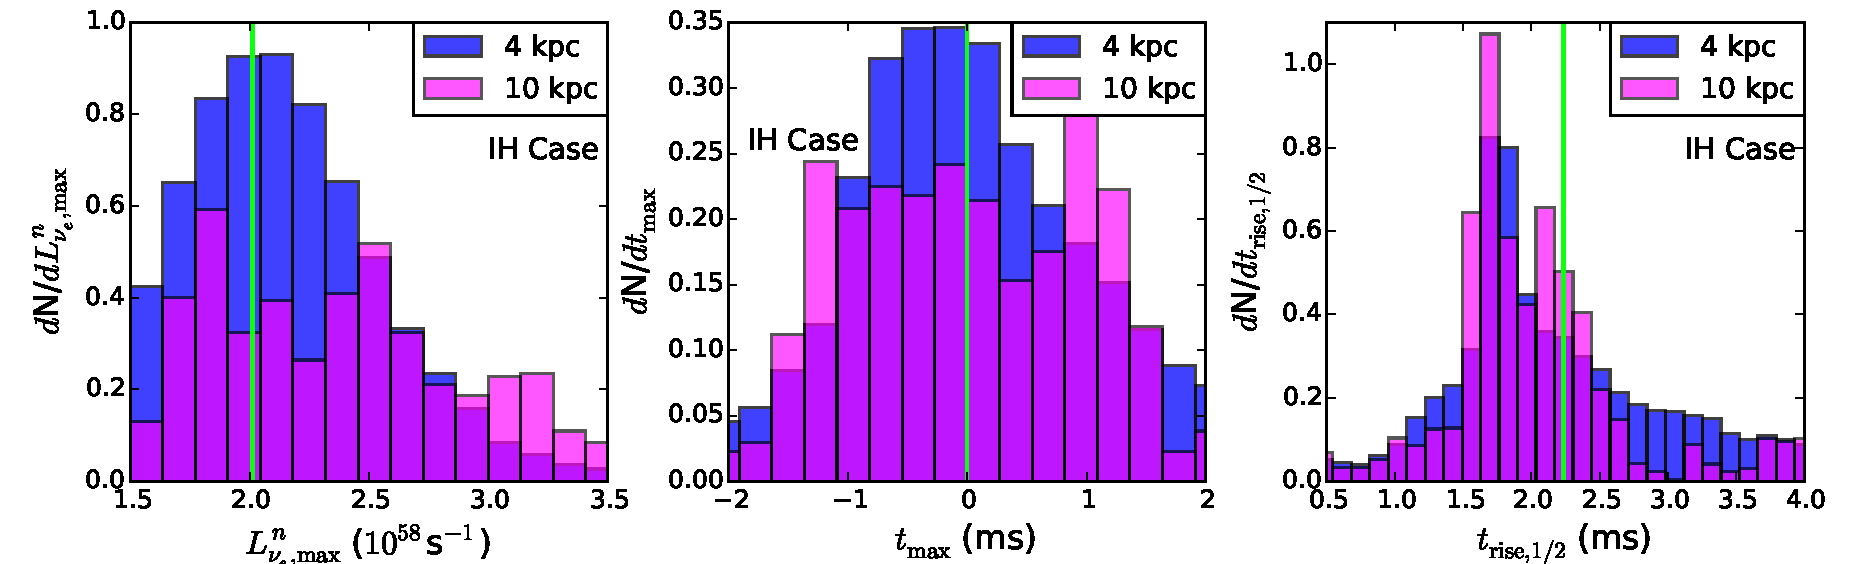
\includegraphics[width=\linewidth]{wh07_15_40g_JUNO_realparameters_histogram_oscillations_backgrounds_IH.pdf}}
\caption{\label{fig:junophysicalparms_hist_ih} Same as
  Figure~\ref{fig:hyperkphysicalparms_hist_ih}, but for JUNO in the
  IH case.  For JUNO, the
  background signals due to IBD's and NC scatterings off of carbon
  have been subtracted.}
\end{figure*}



\begin{figure*}[h]
\centerline{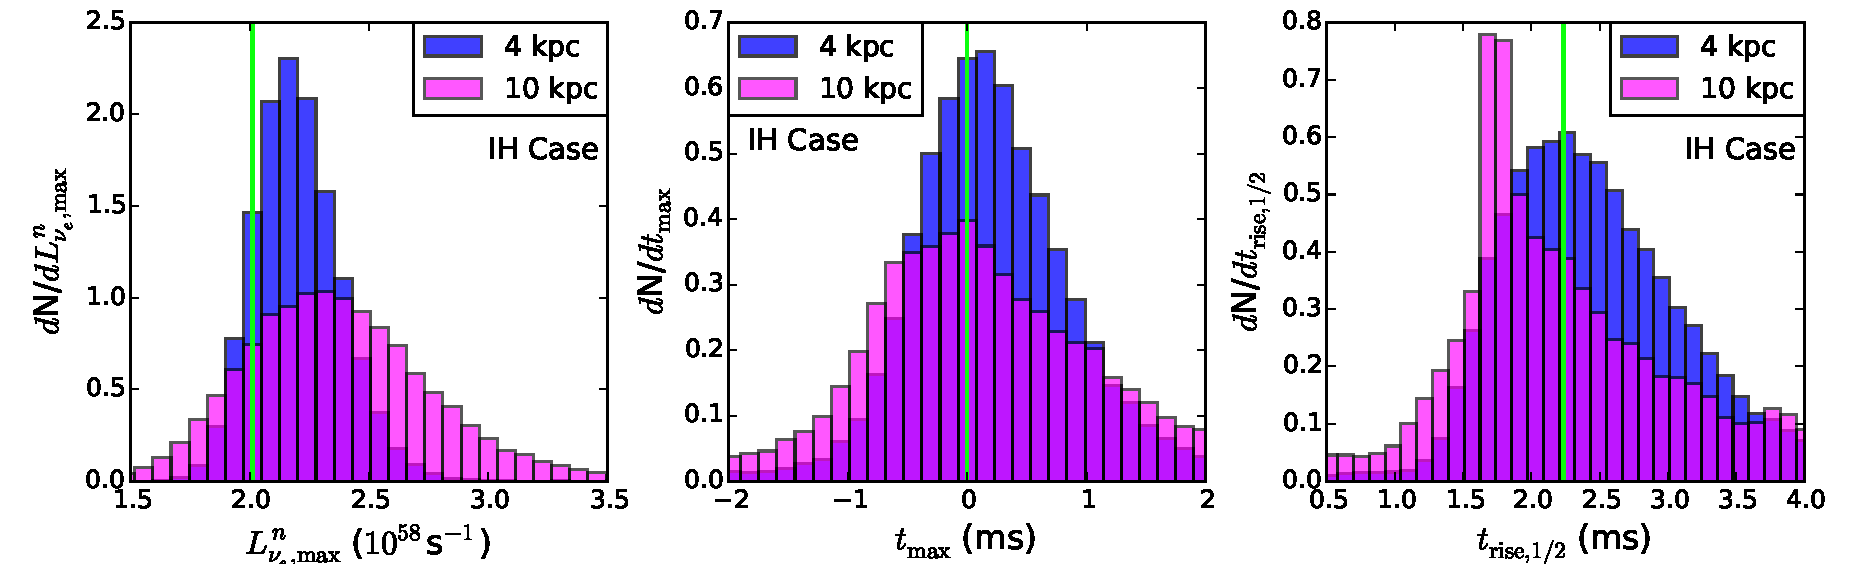
\includegraphics[width=\linewidth]{wh07_15_40g_DUNE_realparameters_histogram_oscillations_backgrounds_IH.pdf}}
\caption{\label{fig:dunephysicalparms_hist_ih} Same as
  Figure~\ref{fig:hyperkphysicalparms_hist_ih}, but for DUNE in the
  IH case.  For DUNE, signals have been subtracted for any detection channel.}
\end{figure*}


\clearpage


\begin{figure*}[h]
\centerline{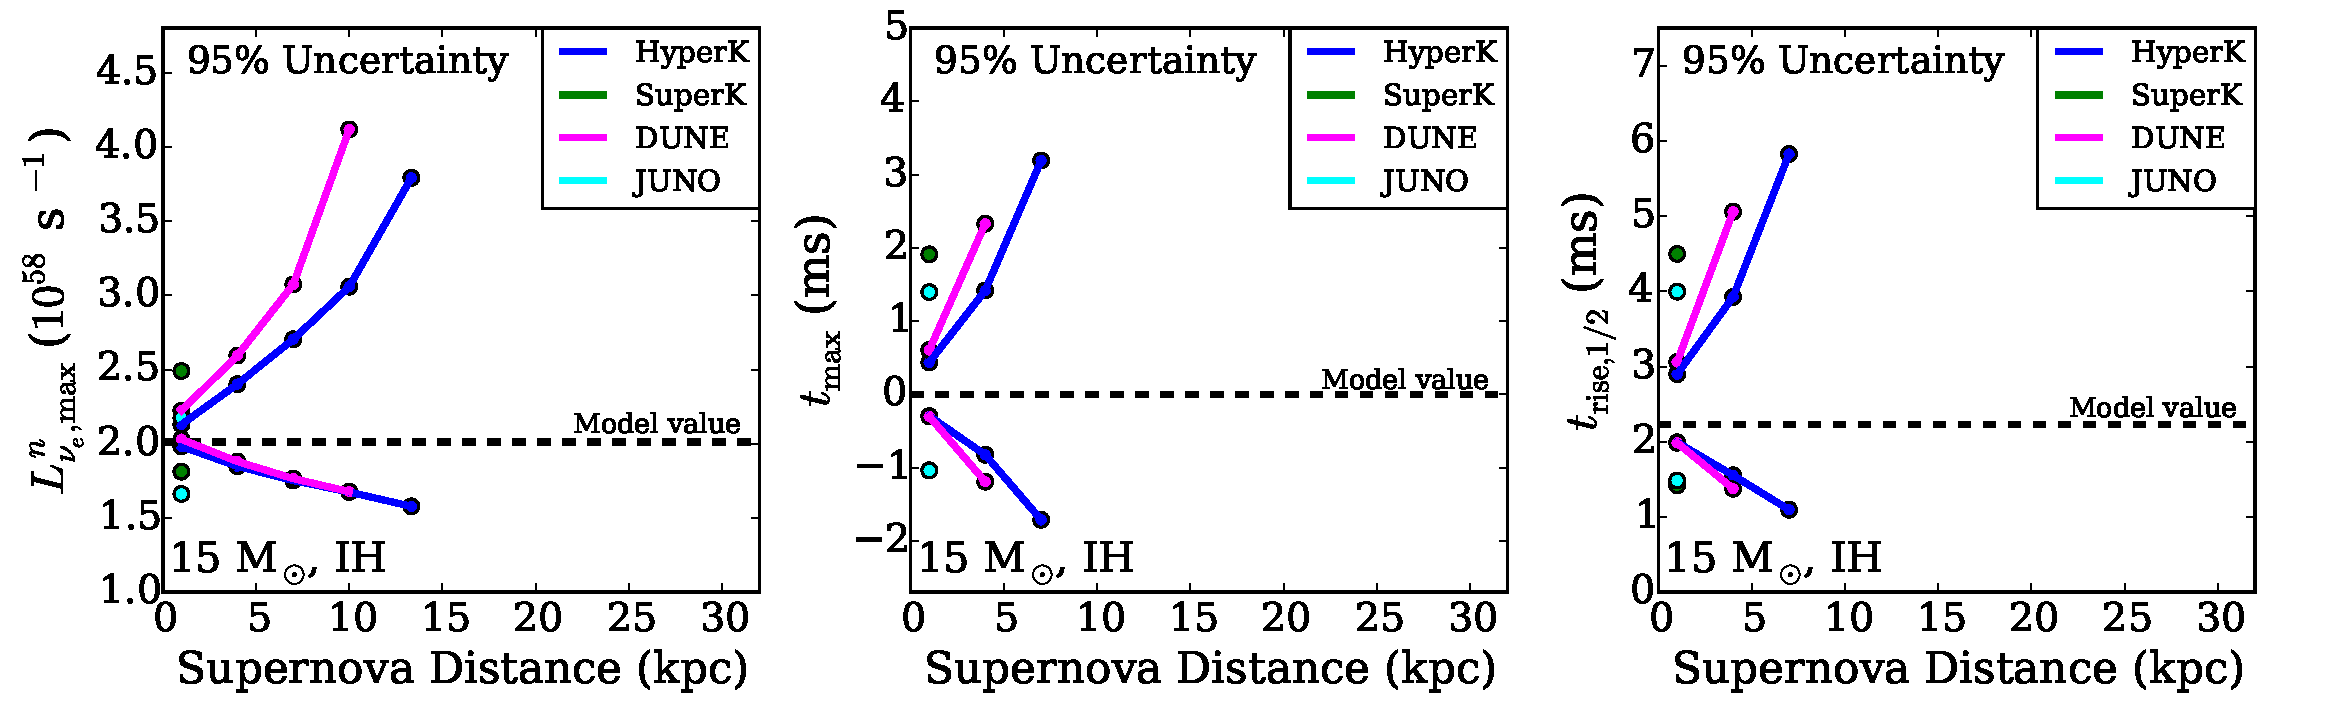
\includegraphics[width=\linewidth]{wh07_15_40g_groupnumber_0_95_funcdistance_backgrounds_oscillations_IH.pdf}}
\caption{\label{fig:15funcD_IH} Similar to
  Figure~\ref{fig:15maxvalfuncD}, but for {\it Left}: \lmax, {\it
    Middle}: \tmax, and {\it
    Right}: \trise, in the no-oscillation case.
  Since IceCube is not able to differentiate neutrino
  types, the \nue\ signal is lost to the \backgrounds\ and so is not
  included in this figure.  
  In all cases, the data for JUNO and/or Super-K are not
  plotted beyond 1 kpc, and the data are shown
  as a single point rather than a line connecting multiple points.
}
\end{figure*}


\setcounter{figure}{0}
\renewcommand{\thefigure}{A\arabic{figure}}

\begin{figure}[h]
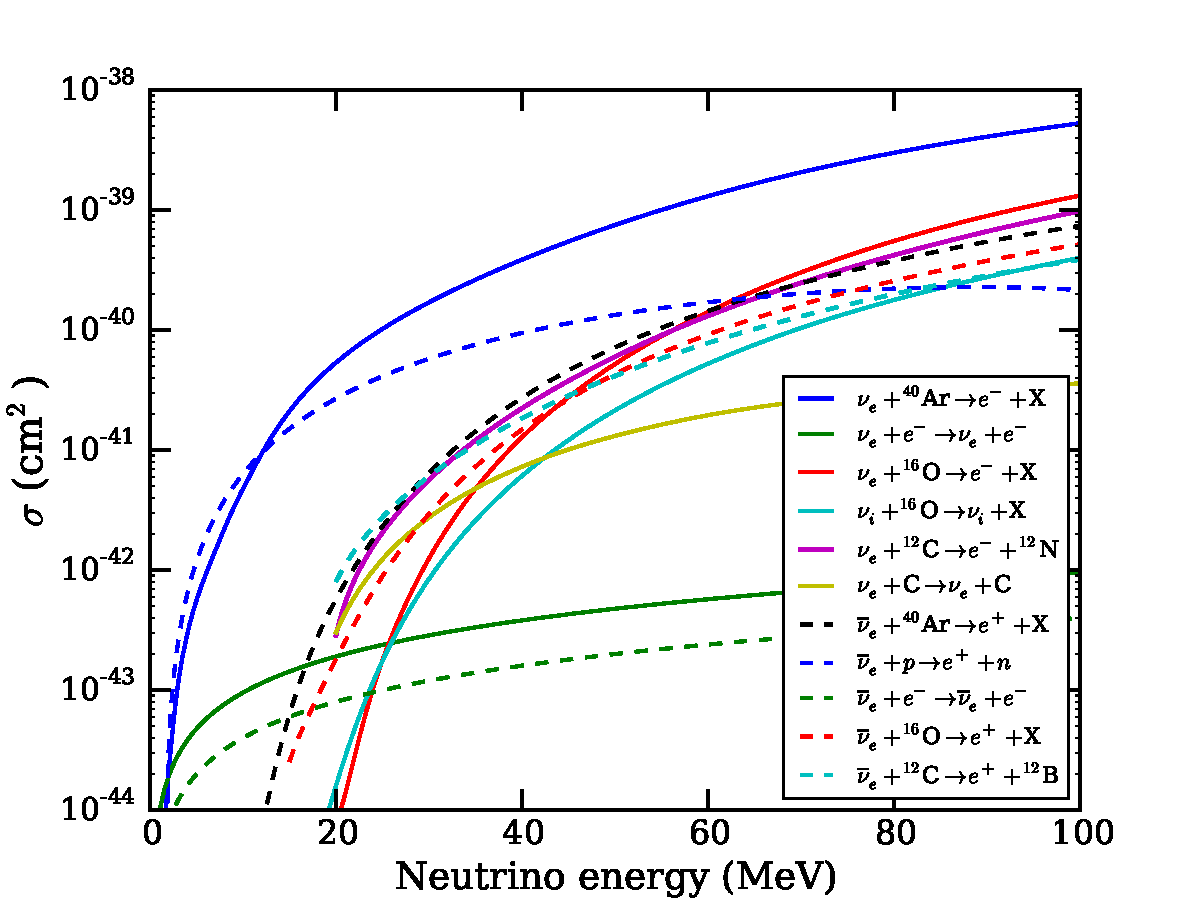
\includegraphics[width=4.5in]{all_neutrino_sigma_for_paper.pdf}
\centering
\caption{\label{fig:sigma}The \nue\ and \anue\ matter-interaction 
cross sections used in  our study over the domain of neutrino 
energies relevant to our study.  The $^{16}$O$(\bar\nu_e,e^+)$X
cross section and both the $^{12}$C cross sections are not plotted to
zero at low energies due to a lack of tabulated data at these energy
values from the sources used.  The cross sections are assumed to be
zero below the lowest extend of the tabulated data.}
\end{figure}
